
% This LaTeX was auto-generated from MATLAB code.
% To make changes, update the MATLAB code and republish this document.

\documentclass{article}
\usepackage{graphicx}
\usepackage{color}

\sloppy
\definecolor{lightgray}{gray}{0.5}
\setlength{\parindent}{0pt}

\begin{document}

    
    \begin{verbatim}
format shortg

Variables=NormGenerate(10000,0,1);
histogram(Variables,'Normalization','pdf')

function Variables = NormGenerate(n,mu,SigmaSquared)
    A=rand((n-mod(n,2))/2+mod(n,2),1);
    B=rand((n-mod(n,2))/2+mod(n,2),1);
    Phi=2*pi*A;
    V=-2*log(1-B);
    X=mu+SigmaSquared*sqrt(V).*cos(Phi);
    Y=mu+SigmaSquared*sqrt(V).*sin(Phi);
    Variables=[X;Y(1:n-(n-mod(n,2))/2-mod(n,2),1)];
end
\end{verbatim}

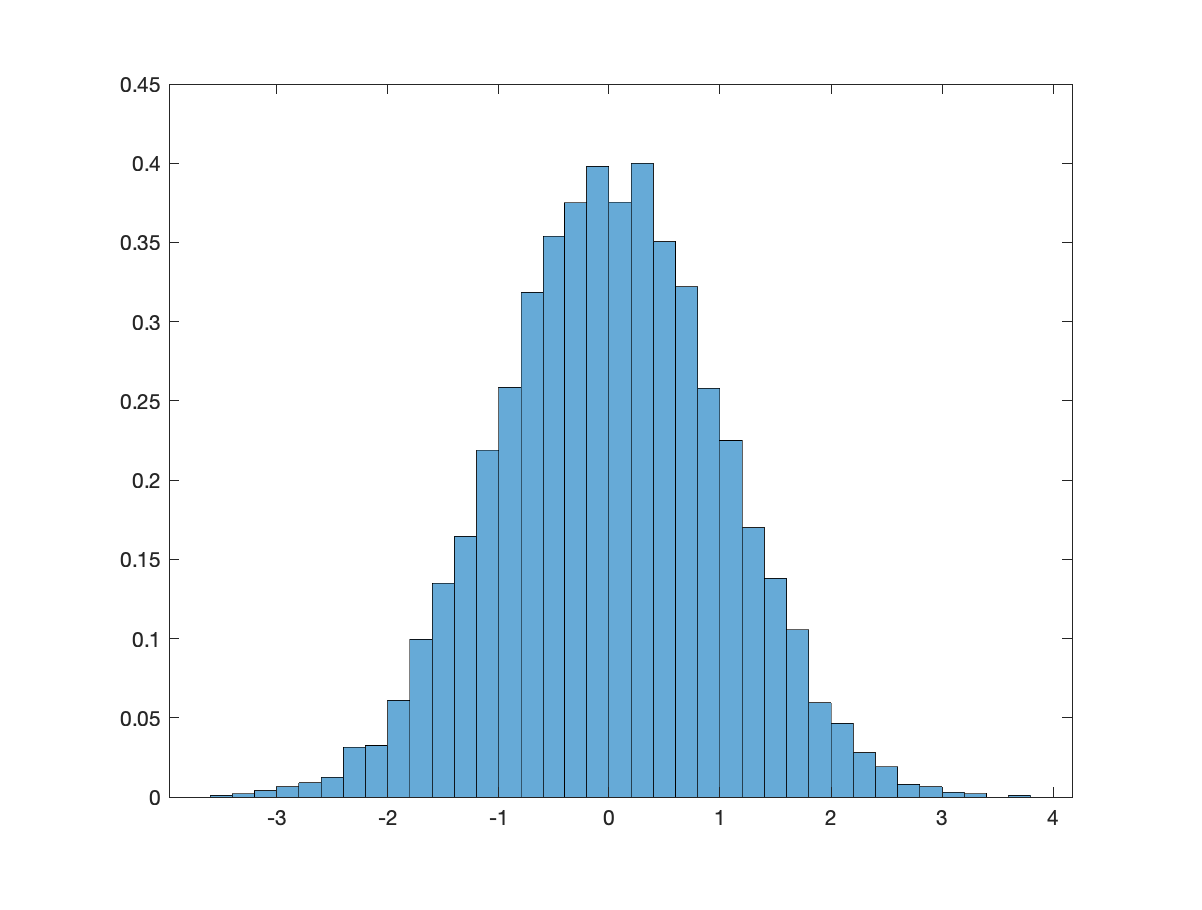
\includegraphics [width=4in]{Code_10_1_01.eps}



\end{document}
    
